\subsection{Inter-Corporate Investments}

\begin{flushleft}
\begin{tabularx}{\textwidth}{p{5em}|p{10.5em}|X|X|p{9.5em}}
\hline
\rowcolor{gray!30}
 & Financial Assets & Associates & Business Combi & Joint Ventures \\
\hline
Influence & Not significant & Significant & Controlling & Shared Control \\
\hline
Interest \% & Usually $< 20\%$ & Usually $20\%$ to $50\%$ & Usually $>50\%$ or other indications of control & \\
\hline
Financial Reporting & Classified as
\xxx Fair value through profit or loss (FVPL)
\xxx Fair value through other comprehensive income (FVOCI)
\xxx Amortised Cost
& Equity Method
& Consolidation
& IFRS: Equity Method \\
\hline
IFRS & IFRS 9 & IAS 28 & IAS 27, IFRS 3, IFRS 10 & IFRS 11, IFRS 12, IAS 28 \\
\hline
GAAP & FASB ASC Topic 320 & FASB ASC Topic 323 & FASB ASC Topics 805 and 810 & FASB ASC Topic 323\\
\hline
\end{tabularx}
\end{flushleft}
\begin{enumerate}[label=\roman*., before=\small]
\setlength{\itemsep}{0pt}
\item IFRS 9 Financial Instruments; IAS 28 Investments in Associates; IAS 27 Separate Financial Statements; IFRS 3 Business Combinations; IFRS 10 Consolidated Financial Statements; IFRS 11 Joint Arrangements; IFRS 12, Disclosure of Interests in Other Entities.
\item FASB ASC Topic 320 [Investments-Debt and Equity Securities]; FASB ASC Topic 323 [Investments- Equity Method and Joint Ventures]; FASB ASC Topics 805 [Business Combinations] and 810 [Consolidations].
\end{enumerate}

\subsubsection{Investment in Financial Assets: IFRS 9}

\begin{figure}[H]
\centering
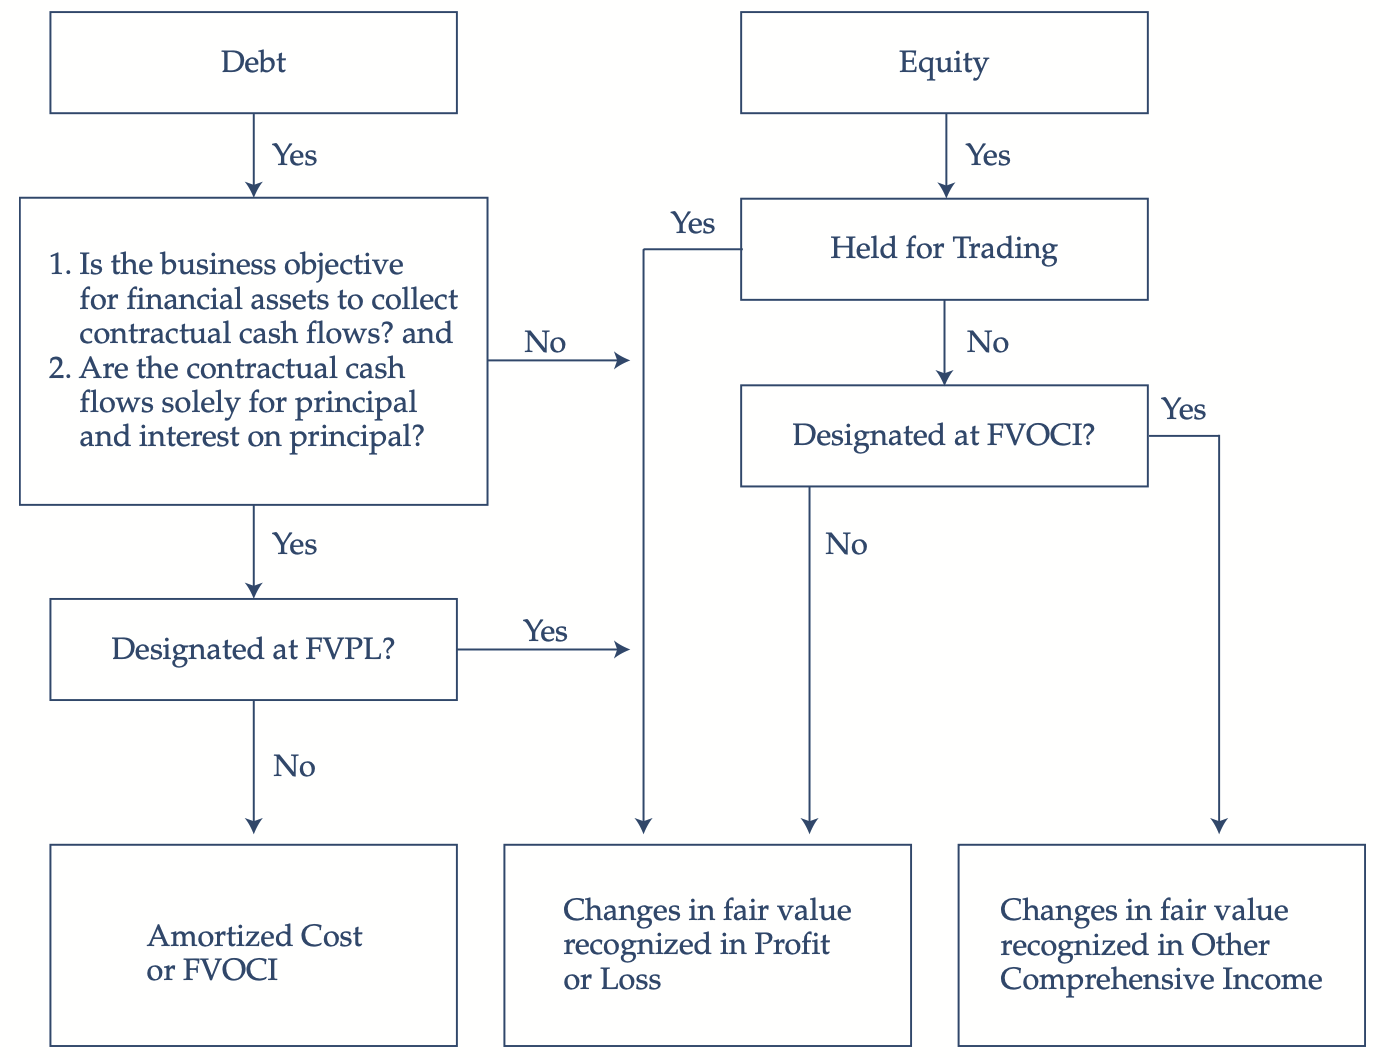
\includegraphics[scale=0.6]{fsa/ifrs9}
\caption{Financial Assets Classification and Measurement Model, IFRS9}
\label{fig:IFRS9}
\end{figure}

\begin{definition} \hlt{Investment in Financial Assets: IFRS 9}\\
IFRS 9 considers contractual characteristics of cash flow and management of financial assets.\\
For loan impairment, expected credit loss model will be used.
\end{definition}

\begin{method} \hlt{Amortised Cost Method - Debt Only}\\
Debt securities meeting following two criteria are accounted for using the amortised cost method:
\begin{enumerate}[label=\roman*.]
\setlength{\itemsep}{0pt}
\item Business Model Test: debt securities are being held to collect contractual cash flows
\item Cash Flow Characteristics Test: the contractual cash flows are principal, or interest on principal, only.
\end{enumerate}
These are reported on the balance sheet at amortised cost - the original cost of debt plus or minus any discount or premium that has been amortised to date.\\
Interest income (coupon cash flow adjusted for amortisation of premium or discount) is recognised in income statement; subsequent changes in fair value are ignored.
\end{method}

\begin{method} \hlt{Fair Value through Profit or Loss - Debt and Equity}
\begin{enumerate}[label=\roman*.]
\setlength{\itemsep}{0pt}
\item Debt: classified as FVPL if held for trading, or if accounting for these securities at amortised cost results in accounting mismatch (inconsistency from different measurement bases for assets and liabilities)
\item Equity: classified as FVPL if held for trading. Otherwise, may be classified as either FVPL or FVOCI, choice is irrevocable.
\item Derivatives: classified as FVPL if not used for hedging. If asset has embedded derivative (i.e., convertible bonds), asset as a whole is valued at FVPL.
\end{enumerate}
Securities are reported on balance sheet at fair value. Changes in fair value (realised and unrealised) are recognised in income statement with any dividend or interest income.
\end{method}

\begin{method} \hlt{Fair Value through Other Comprehensive Income - Debt and Equity}\\
Securities are reported on balance sheet at fair value; any unrealised gain or loss is reported on OCI.\\
Realised gains or losses, dividends, interest income are reported on the income statement.
\end{method}

\begin{flushleft}
\begin{tabularx}{\textwidth}{p{5em}|p{14.5em}|X|p{16em}}
\hline
\rowcolor{gray!30}
 & Amortised Cost & FVPL & FVOCI \\
\hline
Balance Sheet & Amortised cost & Fair Value & Fair value, with unrealised gains and losses (GL) recognised in equity \\
\hline
Income Statement & Interest (including amortisation) & Interest & Interest \\
& & Dividends & Dividends \\
& Realised GL & Realised GL & Realised GL \\
& & Unrealised GL & \\
\hline
\end{tabularx}
\end{flushleft}

\begin{method} \hlt{Reclassification under IFRS 9}
\begin{enumerate}[label=\roman*.]
\setlength{\itemsep}{0pt}
\item Debt: permitted only if business model has changed such that it significantly affects operations.
\item Equity: not permitted, as initial designation is irrevocable.
\end{enumerate}
\end{method}

\begin{method} \hlt{Loan Impairment under IFRS 9}\\
Incurred loss model for loan impairment replaced by expected credit loss model. Require companies to evaluate current and historical information on loan performance (loan commitments and lease receivables), and also forward-looking information.\\
Results in earlier recognition of loan impairment (12 month expected losses for performing loans, lifetime expected losses for non-performing loans).
\end{method}

\subsubsection{Investment in Associates: Equity Method}

\begin{remark} \hlt{Signs of Significant Influence}
\begin{enumerate}[label=\roman*.]
\setlength{\itemsep}{0pt}
\item Investment ownership between 20\% and 50\%
\item Representation on board of directors
\item Participation in the policy-making process
\item Material transactions between investor and investee
\item Interchange of managerial personnel
\item Technological dependency
\end{enumerate}
\end{remark}

\begin{method} \hlt{Equity Method}
\begin{enumerate}[label=\roman*.]
\setlength{\itemsep}{0pt}
\item Initial investment recorded at cost as non-current asset on BS.
\item Carrying amount of investment adjusted to recognise proportionate share of Profit and Loss (PnL); the PnL are recorded on IS.
\item Dividends and other distributions from investee is return of capital, reduce carrying amount of investment on BS, but not reported in investor PnL on IS.
\item On investee loss, investor will receive proportionate share of the loss, reducing the investment account, lower earnings in investor IS.
\item If investment value reduced to zero, equity method is discontinued; further losses will not be recorded. If investee subsequently reports profits, equity method is resumed after investor’s share of profit exceed the share of losses not recognised during the suspension period.
\end{enumerate}
\end{method}

\begin{remark} \hlt{Fair Value Option}
\begin{enumerate}[label=\roman*.]
\setlength{\itemsep}{0pt}
\item GAAP: allows investments to be recorded at fair value.
\item IFRS: fair value option only available to VC, mutual funds, unit trusts, ILPs etc. 
\end{enumerate}
Decision to use fair value option is irrevocable; any changes in value (with dividends) are recorded in IS.\\
Investor investment account on BS do not reflect proportionate share of PnL, dividends or other distributions. Excess of cost over fair value of investee identifiable net assets is not amortised, nor is goodwill created.
\end{remark}

\begin{remark} \hlt{Excess of Purchase Price over Book Value Acquired}
\begin{enumerate}[label=\roman*.]
\setlength{\itemsep}{0pt}
\item At acquisition, the difference is first allocated to specific assets and liabilities (AnL) of assets using fair values, accounted in manner consistent with accounting treatment for the specific AnL to which it is assigned. Amounts allocated to AnL which are expensed or depreciated to be similarly treated. \\
Initially the BS records the cost in the investment account.
\item The difference is then amortised to proportionate share of investee PnL over economic lives of the assets (whose fair value exceeds book value).\\
On the BS, as the differences are amortised, the balance in investment account will converge to proportionate share of book value of net assets of the associate.\\
Investor record these adjustments by reducing carrying amount of investment on BS and reducing investee profit recognised on its IS.
\item The goodwill is reviewed for impairment on regular basis. This is included in carrying amount of the investment on the investor BS.
\end{enumerate}
\end{remark}

\begin{method} \hlt{Investor Balance Sheet Impact: Equity Method}
\begin{align}
\text{Purchase Price} - \text{\% share of net asset BV} &= \text{Excess of purchase price} \nonumber \\
\text{Excess of purchase price} - \text{\% share of (FV} -  \text{BV) of PPE} &= \text{Goodwill} \nonumber \\
\text{Investor \% share of investee net income} - \text{Depreciation of \% share of excess PPE} &= \text{Equity income} \nonumber \\
\text{Investment balance beginning} + \text{Equity income} - \text{\% share of dividends} &= \text{Investment balance end} \nonumber
\end{align}
\end{method}

\begin{method} \hlt{Investor Income Statement Impact: Equity Method}
\begin{align}
\text{Impact} = \text{Equity income} - \text{\% share of unrealised profit from downstream and upstream sale} \nonumber
\end{align}
\end{method}

\begin{remark} \hlt{Treatment of PPE Depreciation on Investor}
\begin{enumerate}[label=\roman*.]
\setlength{\itemsep}{0pt}
\item IFRS: PPE is to be carried at either historical cost or fair value (less accumulated depreciation)
\item GAAP: PPE is to be carried at historical cost (less accumulated depreciation) only
\end{enumerate}
\end{remark}

\begin{method} \hlt{Impairment of Investments}\\
IFRS and GAAP require periodic reviews for impairment. If fair value of investment is less than carrying value permanently, impairment loss is recognised.
\begin{enumerate}[label=\roman*.]
\setlength{\itemsep}{0pt}
\item IFRS: require objective evidence due to one or more loss events that occur after initial recognition, and the loss event has impact on future CF reliably estimated.\\
Entire carrying amount tested by comparing recoverable amount with carrying amount.\\
Impairment loss recognised on IS; carrying amount on BS reduced directly or through allowance account.\\
Reversal of impairment loss allowed to extent that recoverable amount of net investment increases.
\item GAAP: treat impairment as permanent.\\
Impairment loss recognised on IS; carrying value of investment on BS reduced to fair value.\\
Prohibit reversal of impairment loss even if fair value later increases.
\end{enumerate}
\end{method}

\begin{remark} \hlt{Transactions with Associates}\\
Investor can influence terms and timing of transactions with associates. Profits from such transactions cannot be realised until confirmed through use or sale to third parties.\\
Investor share of unrealised profit deferred by reducing amount recorded under equity method. When deferred profit is confirmed, added this to equity income based on recorded values in associate’s accounts.
\begin{enumerate}[label=\roman*.]
\setlength{\itemsep}{0pt}
\item Upstream (investee to investor): profit recorded on investee IS as PnL. Investor’s share of unrealised profit is thus included in equity income on investor IS.\\
However, for profit that is unconfirmed (goods not been used or sold by investor), investor must eliminate proportionate share of profit from equity income of investee.
\item Downstream (investor to investee): profit recorded on investor IS. Investor must eliminate proportionate share of profit that is unconfirmed. Adjust equity income on investor’s IS by deducting on share percent.
\end{enumerate}
\end{remark}

\begin{remark} \hlt{Disclosures from Transactions with Associates}\\
Investee results are included in investor’s accounts with time lag (not more than one quarter). Dividends from investee are not included in investor income.\\
In consolidated BS, book value of shareholdings in investee is increased by investor’s share of associate net income, reduced by amortisation of surplus values and amount of dividends received.
\end{remark}

\begin{remark} \hlt{Analytical Issues of Equity Method}
\begin{enumerate}[label=\roman*.]
\setlength{\itemsep}{0pt}
\item Degree of control of investor on investee may not be proportional to shareholdings.
\item Significant AnL of investee are not reflected on investor BS, which affect debt ratios. Net margin ratios may be overstated as income for investee is included in investor net income, but not in sales.
\end{enumerate}
When analysing associates, consider quality of equity method earnings, potential restriction on dividend CF.
\end{remark}

\subsubsection{Business Combinations: Consolidation}

\begin{definition} \hlt{Types of Business Combinations}
\begin{enumerate}[label=\roman*.]
\setlength{\itemsep}{0pt}
\item \hlt{Merger}: Target 100\% absorbed. Net assets of Company B transferred to Company B.
\begin{equation}
\text{Company } A + \text{Company } B = \text{Company } A \nonumber
\end{equation}
\item \hlt{Acquisition}: Companies connected by parent-subsidiary relationship. May acquire less than 50\% and still exert control. May acquire less than 100\%, and non-controlling (minority) shareholder interest reported on consolidated financial statements.
\begin{equation}
\text{Company } A + \text{Company } B = (\text{Company } A + \text{Company } B) \nonumber
\end{equation}
\item \hlt{Consolidation}: New legal entity formed, take over net assets of both companies. 
\begin{equation}
\text{Company } A + \text{Company } B = \text{Company } C \nonumber
\end{equation}
\end{enumerate}
IFRS: no distinction made among business combinations.\\
GAAP: classified as merger, acquisition, or consolidation.
\end{definition}

\begin{method} \hlt{Pooling-of-Interests Method (IFRS Defunct)}\\
Ownership interest of two firms combined, participants viewed as equals.
\begin{enumerate}[label=\roman*.]
\setlength{\itemsep}{0pt}
\item Two firms asset and liabilities combined using historical book values
\item Operating results for prior periods restated as though the two firms were always combined
\item Ownership interests continue, former accounting bases are maintained
\end{enumerate}
\end{method}

\begin{method} \hlt{Acquisition Method: Recognition and Measurement}\\
Fair value of target includes acquisition-date fair value of any contingent consideration. Direct costs of business combination are expensed. Recognition and measurement of:
\begin{enumerate}[label=\roman*.]
\setlength{\itemsep}{0pt}
\item Identifiable assets and liabilities: measure at fair value at date of acquisition, including intangible assets
\item Contingent liabilities (CL): measure if it is a present obligation from past events, can be measured reliably.
\begin{enumerate}[label=\arabic*.]
\setlength{\itemsep}{0pt}
\item IFRS: includes CL if fair values can be reliably measured.
\item GAAP: only includes CL that are probable and can be reasonably measured.
\end{enumerate}
\item Indemnification assets (IA): recognise IA if seller contractually indemnifies acquirer for outcome of a contingency or uncertainty related to all or part of a specific asset or liability of the seller. Seller may also indemnify acquirer against losses above a specified amount on a liability arising from a particular contingency. Acquirer will recognise the IA at the acquisition date fair value.
\item Financial assets and liabilities: identifiable AnL are classified according to IFRS and GAAP standards. Acquirer reclassifies financial AnL based on contractual terms, economic conditions, acquirer’s operation and accounting policies.
\item Goodwill: GAAP requires full goodwill. IFRS prefers partial goodwill; full can be used. IFRS allows recognition on transaction-by-transaction basis. 
\begin{enumerate}[label=\arabic*.]
\setlength{\itemsep}{0pt}
\item Partial Goodwill: acquisition price less acquirer’s share of fair value of all tangible and intangible AnL, CL acquired. \begin{align}
\text{Partial Goodwill} &= \text{Acquisition Price} - \text{\% share of fair value of net identifiable assets} \nonumber \\
\text{Partial Goodwill} &= \text{Acquirer \% share of equity} \times \text{Full Goodwill} \nonumber \\
\text{Non-Controlling Interest} &= \text{\% share of NCI} \times \text{Acquiree fair value of identifiable net assets} \nonumber
\end{align}
\item Full Goodwill: fair value of entity less fair value of all tangible and intangible AnL, CL 
\begin{align}
\text{Full Goodwill} &= \text{Fair value of combined entity} - \text{fair value of net identifiable assets} \nonumber \\
\text{Non-Controlling Interest} &= \text{\% share of NCI} \times \text{Fair value of entity} \nonumber
\end{align}
\end{enumerate}
\item Bargain purchase: when acquisition price is less than fair value. Difference to be recognised immediately in PnL on IS. Any contingent consideration is measured and recognised at fair value; subsequent changes in value are recognised in PnL.
\end{enumerate}
\end{method}

\begin{remark} \hlt{Full Goodwill vs Partial Goodwill} \\
Full goodwill results in higher total assets and higher total equity than partial goodwill.\\
ROA and ROE will be lower if full goodwill method is used.
\end{remark}

\begin{method} \hlt{Investor Balance Sheet Impact: Acquisition Method}
\begin{align}
\text{End current assets} &= \text{Beginning current assets} + \text{acquiree current assets} - \text{acquisition cash fee} \nonumber \\
\text{End current liabilities} &= \text{Beginning current liabilities} + \text{acquiree current liabilities} \nonumber \\
\text{Minority Interest in Equity} &= \text{\% share of NCI} \times \text{Subsidiary equity} \nonumber
\end{align}
\end{method}

\begin{method} \hlt{Investor Income Statement Impact: Acquisition Method}
\begin{align}
\text{End revenue} &= \text{Beginning revenue} + \text{acquiree revenue} \nonumber \\
\text{End expenses} &= \text{Beginning expenses} + \text{acquiree expenses} \nonumber \\
\text{Minority Interest} &= - \text{\% share of NCI} \times \text{acquiree net income} \nonumber
\end{align}
Acquisition method results in higher revenue and expenses, but net income is the same.
\end{method}

\begin{method} \hlt{Goodwill Impairment}
\begin{enumerate}[label=\roman*.]
\setlength{\itemsep}{0pt}
\item IFRS: At acquisition, total goodwill recognised is allocated to each of acquirer’s cash generating units (lowest level within combined entity monitored for impairment purposes) that will benefit from expected synergies due to the combination with the target.\\
Impairment testing under one-step approach: If recoverable amount < carrying value of cash-generating unit, then impairment loss is recognised. 
\begin{equation}
\text{Impairment Loss} = \text{Carrying value of unit} - \text{Recoverable amount of unit} \nonumber
\end{equation}
Impairment loss is first applied to goodwill allocated to cash-generating unit; if reduced to zero, remaining amount allocated to other non-cash assets in the unit on pro-rata basis.
\item GAAP: At acquisition, total goodwill allocated to each of acquirer’s reporting units (operating segment or component of operating segment that is one level below operating segment as a whole).\\
Impairment testing under two-step approach: 
\begin{enumerate}[label=\arabic*.]
\setlength{\itemsep}{0pt}
\item If fair value < carrying value of reporting unit (with goodwill), potential impairment identified.
\begin{equation}
\text{Implied goodwill} = \text{Fair value of unit} - \text{Fair value of unit identifiable net assets} \nonumber
\end{equation}
\item Impairment loss is difference between carrying value of goodwill and implied fair value of goodwill.
\begin{equation}
\text{Impairment loss} = \text{Carrying value of goodwill} - \text{Implied goodwill} \nonumber
\end{equation}
\end{enumerate}
Impairment loss then applied to goodwill allocated to reporting unit; if reduced to zero, no other adjustment made to carrying value of any of reporting unit’s other AnL. Prudent to test other asset values for recoverability and possible impairment.
\end{enumerate}
IFRS and GAAP: impairment loss is recorded as separate line item in IS.
\end{method}

\subsubsection{Joint Ventures: Equity Method, Consolidation Method}

\begin{remark} \hlt{Purpose of Joint Ventures (JV)}\\
For entering foreign markets, conduct specialised activities, engage in risky projects.\\
May be primarily contractual relationships or common ownership of assets.\\
Can be partnerships, LLCs (corps) or other legal forms (unincorporated associations).\\
IFRS identify the characteristic of JVs as follows: a contractual agreement exists between two or more venturers, and the contract establishes joint control.
\end{remark}

\begin{method} \hlt{Equity Method vs Consolidation Method}
\begin{enumerate}[label=\roman*.]
\setlength{\itemsep}{0pt}
\item Proportional consolidation: require venturer’s share of assets, liabilities, income, expenses of JV to be combined or show on line-by-line basis with similar items under its sole control.
\item Equity method: line item 'equity in income of JV' on IS, line item 'investment in JV' on BS.
\end{enumerate}
Proportionate consolidation results in higher AnL, but stockholder's equity and net assets is the same. Proportionate consolidation also results in higher revenues and expenses, but net income is the same.
\end{method}

\subsubsection{Special Purpose Entities, Variable Purpose Entities}

\begin{remark} \hlt{Purpose of Special Purpose Entities (SPEs)}\\
Sponsor transfers assets to SPE, obtains right to use assets held by SPE, or perform services for the SPEs. Third party provide funding to the SPE.\\
Third party interest may take form of debt, equity, participation right, or residual interest in a lease. Sponsor retains significant beneficial interest, even if it may own little or none of SPE’s voting equity.\\
For segregation of certain activities, hence reduce risk and lower cost of financing.\\
Typically structured such that sponsor has control over SPE finances or operating activities, and third parties have controlling interest in SPE equity.
\end{remark}

\begin{remark} \hlt{IFRS Sponsor Control of SPEs}\\
IFRS require consolidation if there is sponsor control, where:
\begin{enumerate}[label=\roman*.]
\setlength{\itemsep}{0pt}
\item Investor has ability to exert influence on financial and operating policy of entity.
\item Investor is exposed, or has rights to variable returns from involvement with entity.
\end{enumerate}
SPEs involved in structured financial transaction will require evaluation of the purpose, design and risks.
\end{remark}

\begin{definition} \hlt{Primary Beneficiary}\\
The party that will absorb the majority of SPE expected losses, receive the majority of SPE expected residual returns, or both.
\end{definition}

\begin{remark} \hlt{GAAP Classification of SPE as VIE}\\
VIE includes other entities besides SPEs. Classifies SPE as VIE if one of the conditions is met:
\begin{enumerate}[label=\roman*.]
\setlength{\itemsep}{0pt}
\item Total equity at risk insufficient to finance activities without financial support from other parties; or
\item Equity investors lack one of the following: 
\begin{enumerate}[label=\arabic*.]
\setlength{\itemsep}{0pt}
\item Ability to make decisions
\item Obligation to absorb losses
\item Right to receive returns
\end{enumerate}
\end{enumerate}
\end{remark}

\begin{method} \hlt{GAAP Consolidation for SPEs and VIEs}
\begin{enumerate}[label=\roman*.]
\setlength{\itemsep}{0pt}
\item SPEs: Require primarily beneficiary to consolidate the SPE regardless of its voting interest in the SPE, or its decision-making authority.\\
Two-component consolidation: variable interest component and voting interest (control) component.
\item VIEs: Primary beneficiary of VIE must consolidate it as subsidiary regardless of how much equity the beneficiary has in VIE. The entity absorbing majority of losses must consolidate the VIE if another entity receive majority of VIE’s expected residual returns. Entities must disclose relationship with VIE even if not the primary beneficiary.\\
Non-controlling interests in the VIE must be shown on the consolidated BS and IS of primary beneficiary. 
\end{enumerate}
\end{method}

\subsubsection{Issues that Impair Comparability}

\begin{remark} \hlt{Contingent Assets and Liabilities}
\begin{enumerate}[label=\roman*.]
\setlength{\itemsep}{0pt}
\item IFRS: contingent assets are never recognised.\\
Contingent liabilities whose fair value can be measured reliably are recognised at time of acquisition. Subsequently, contingent liabilities measured at the higher of value initially recognised or best estimate of amount needed to settle.
\item GAAP: Contractual contingent AnL recorded at fair value at date of acquisition. Non-contractual contingent AnL also recorded if 'more likely than not' they meet the definition of an asset or liability.\\
Subsequently, contingent liabilities are measured at higher of amount initially recognised, or best estimate of amount of the loss. Contingent assets are measured at lower of acquisition date fair value or best estimate of the future settlement amount.
\end{enumerate}
\end{remark}

\begin{remark} \hlt{Contingent Consideration}\\
If terms of acquisition involve contingent consideration, this is recognised at fair value under both IFRS and GAAP as an asset, liability, or equity.\\
Subsequent changes in fair value are recognised in income statement, unless value was originally classified in equity (any changes settle within equity and not on IS).
\end{remark}

\begin{remark} \hlt{In-Process R\&D}\\
In-Process R\&D is capitalised as separate intangible asset, measured at fair value (if can be measured reliably).\\
In subsequent periods, this is subject to amortisation if fully completed, or impairment if no product results or if product is not technically and/or financially viable.
\end{remark}

\begin{remark} \hlt{Restructuring Costs}\\
IFRS and GAAP do not recognise restructuring costs. This is recognised as an expense in the periods the restructuring costs are incurred.
\end{remark}

\begin{remark} \hlt{Choice of Accounting Method on BS and IS Items}
\begin{enumerate}[label=\roman*.]
\setlength{\itemsep}{0pt}
\item Net Income: same for all three methods
\item Equity: Equity method and proportionate consolidate has same equity. Acquisition method equity will be higher by amount of minority interest.
\item Assets and Liabilities: highest under acquisition method, lowest under equity method.
\item Revenues and Expenses: highest under acquisition method, lowest under equity method.
\end{enumerate}
\end{remark}

\begin{flushleft}
\begin{tabularx}{\textwidth}{p{8em}|p{17.5em}|p{10em}|X}
\hline
\rowcolor{gray!30}
 & Equity & Prop Cosol & Acquisition \\
\hline
Net Profit Margin & Higher (sales lower, net income same) & In-Between & Lower \\
\hline
ROE & Higher (equity lower, net income same) & Same as equity method & Lower \\
\hline
ROA & Higher (net income same, assets lower) & In-Between & Lower \\
\hline
\end{tabularx}
\end{flushleft}